\documentclass[printmode]{mgr}

\usepackage[utf8]{inputenc}
\usepackage[T1]{fontenc}

\usepackage{pdflscape}
% https://en.wikibooks.org/wiki/LaTeX/Source_Code_Listings
\usepackage{listings}
\lstset{
  frame=single,
  language=Bash
}

\usepackage{graphicx}
\usepackage{caption}
\usepackage{subcaption}
\usepackage{psfrag}
\graphicspath{{./images/}}

\usepackage{amsmath}
\usepackage{amsfonts}

\usepackage{supertabular}
\usepackage{array}
\usepackage{tabularx}
\usepackage{hhline}

\usepackage{hyperref}

\title{Embedded Linux \\ build systems}
\engtitle{Systemy implementacji \\ wbudowanego Linuxa}
\author{Cezary Dynak}
\supervisor{dr Witold Paluszyński}

\field{Automatyka i~Robotyka (AIR)}
\specialisation{Embedded Robotics (AER)}

\begin{document}
\bibliographystyle{plabbrv}

\maketitle
\dedication{6cm}{To my wife and son}

\tableofcontents

\chapter{Introduction}
\section{Goals of the project}
The goal of this project is to explore, compare and extend embedded Linux build systems. \cite{web:bis-org-pl}
\begin{figure}[htbp]
  \centering
    
\includegraphics[width=0.5\textwidth]{Tux.png}
  \caption{Penguin Tux - Linux mascot}
  \label{fig:panel-dotykowy}
\end{figure}



\chapter{Linux build systems for embedded devices}
\label{chapter:build systems}
% https://www.embarcados.com.br/embedded-linux-build-systems/
% https://en.wikipedia.org/wiki/Menuconfig
% official repository / github mirror / download directory


\section{Basic definitions}

Despite that every aspect of computing could be described by numbers and mathematical operations, unfortunately the naming conventions could be misleading, especially in the area which I'm describing. People understand the word "Linux" differently in different context, as there is also never ending debate about the term "GNU/Linux". Sometimes some buzzwords like "cloud" and "IoT" are strongly promotes by the business, which makes common understanding even more blurred. Therefore, I would like to explain how to interpret the key wording.

\paragraph{Operating system}

\paragraph{Operating system kernel}

\paragraph{Linux} is an open source operating system kernel, that follow the POSIX standards. Initial release takes place in 1991 and since then it is being developed by thousands of voluntary collaborators as well as major IT companies. Formerly it was compatible only with x86 standard processor architecture for personal computers, but to others, especially ARM that is used by the most of mobile and embedded devices. The work of its creator Linux Torvalds and lead maintainer Greg Kroah-Hartman is currently sponsored by the Linux Foundation. As for 2018, all of the world fastest supercomputers from TOP 500 ranking are using this kernel.

\paragraph{Linux distribution} is an operating system, that uses he Linux kernel.

\paragraph{Embedded device}

\paragraph{Cross-compilation}

\paragraph{Embedded Linux build system} is a set of software development tools, that enables creation of Linux distribution within the process of cross-compilation and produces complete operating system image, to be deployed on an embedded device.

\section{Problem of definition}
There is much confusion in semantic layer here. Linux is just a operating system kernel, it doesn't providing any user space.
In the beginning, when it was created, there was no distributions, so if anybody want to utilize it, it had to be compiled and configured in a way later described in Linux From Scratch. After some conceptual projects, the two still most important distributions were created: Debian and Red Hat. They provides not only fully working solution, but also their own way to adding software - package management systems: deb and rpm. \\
It could be clearly said, that Linux distribution is a complete operating system, which includes certain set of software and distribution maintainers take care about preparing release version for certain hardware. Nevertheless, distributions are mostly used on personal computers, that have very standardized x86-based hardware, while embedded platforms differ very much between each other. The base idea behind distributions is that user is able to extend it and tune to own needs, while embedded systems mostly cope with non-human interfaces and need to be strongly pre-configured. \\
The lines are blurred in this area, but I will suggest using therm "embedded Linux build systems" for every set of tools, that makes it possible to create complete operating system with Linux kernel on embedded device - starting with building from source for another CPU architecture and ending with complete disk image containing bootloader, kernel and root file system. Within this umbrella therm some project identifies themselves differently as "distribution creators" or "executable documentation", but they share the same goal.

\section{Common aspects}

\begin{landscape}

\begin{table}
  \begin{tabular}{| p{2.5cm} | p{3cm} | p{3cm} | p{3cm} | p{3cm} | p{3cm} | p{3cm} |}
    \hline
    name & Raspberry Pi 1 & BeagleBone Black & PandaBoard & Wandboard Quad & Grinn liteboard & Asus Eee PC 1215n \\
    \hline
    Buildroot & raspberrypi \_defconfig &  beaglebone \_defconfig & pandaboard \_defconfig & wandboard \_defconfig & grinn\_liteboard \_defconfig & pc\_x86\_64\_efi \_defconfig \\
    \hline
    LEDE & & & & & & \\
    \hline
    LTIB & & & & & & \\
    \hline
    Pengutronix & & & & & & \\
    \hline
    Yocto & & & & & & \\
    \hline
  \end{tabular}
\end{table}

\end{landscape}

\section{Differences}

\subsection{Buildroot}
% https://www.slideshare.net/tpetazzoni/buildroot-building-embedded-linux-systems-made-easy-linux-conf-australia-2014
% https://events.linuxfoundation.org/sites/events/files/slides/belloni-petazzoni-buildroot-oe_0.pdf
% http://linuxgizmos.com/free-embedded-linux-training-materials-demystify-buildroot/

Buildroot is a simple and fast tool that enables to build a complete Linux embedded system by means of cross-compilation. During the building process a cross-compilation toolchain, a root filesystem, a Linux kernel and a boot loader can be generated.  Furthermore, each of these steps can be performed separately.

\subsection{OpenWRT / LEDE}

OpenWrt is a Linux distribution designed for embedded devices, commonly used on home routers. It gives users a possibility to make a fully customized operating system that is not dependent on firmware supplied by vendor. However, in May 2016  a group of developers decided to fork the project and create LEDE - Linux Embedded Development Environment.

\subsection{LTIB}
% http://ltib.org/home-intro 
% http://ltib.org/pages/LTIB_generic_v1.4_-_version_6.4.1.pdf

% http://www.bitshrine.org/autodocs/LtibFaq.html#ref_10
% What is required on your host before installing LTIB

Linux Target Image Builder is a tool which allows to develop and deploy BSPs on target platforms. It was launched and financed by Freescale Seminconductor as  and then transferred to Savannah. According to that, a Linux system can be built with a use of packages from the common pool.

\subsection{Pengutronix / PTXdist}
% http://elinux.org/PTXdist
% http://public.pengutronix.de/oselas/bsp/pengutronix/OSELAS.BSP-Pengutronix-Generic-arm-Quickstart.pdf
% http://public.pengutronix.de/oselas/toolchain/
% http://public.pengutronix.de/software/ptxdist/
% http://public.pengutronix.de/software/ptxdist/appnotes/
% https://git.pengutronix.de/cgit/DistroKit

% https://www.mail-archive.com/ptxdist@pengutronix.de/msg10260.html
% Difference between DIstroKit and OSELAS.BSP-Pengutronix-Generic

PTXdist is a build system that creates embedded Linux distributions directly from the source code. It is led by German company Pengutronix and supposed to maximize control and long-term maintainability. It starts with a cross toolchain and then next steps lead to packed binary image.

\subsection{Yocto}

Yocto is a set of tools and templates that enables to generate an operating system images for embedded Linux systems. The process is independent of the hardware architecture. Yocto includes core system components such as BitBake, OpenEmbedded-Core and Poky. 

\subsection{LFS}

\url{http://www.linuxfromscratch.org}\\
\url{http://trac.clfs.org}\\
\url{http://intestinate.com/pilfs/}\\
\url{https://raspberrypi.stackexchange.com/questions/25/is-there-a-linux-from-scratch-lfs-arm-equivalent}

\subsection{Distribution custom systems}

multistrap?

\subsection{Comercial / Closed Source}

windriver?

\section{Development boards}
\label{section:development-boards}

From the beginning of embedded systems history, microprocessor development boards were just a training resource for engineers.
Usually they were designed and produced by companies that have created certain chip and costs a lot of money, that it was not affordable for hobbyists or students.
In recent years this state has been changed by a few factors:
\begin{itemize}
  \item the spread of ARM architecture micro-controllers with efficiency comparable to personal computers (1GHz),
  \item creating development boards by community as open hardware, that resulted in cost reduction,
  \item adding peripherals specific not for embedded systems but for personal computers.
\end{itemize}
This led to discovering totally new use cases for development boards which explode due to widespread success of Raspberry Pi platform. \\
I have selected some of most popular devices with ARM to compare them, but also included my personal laptop computer as a reference for x86 architecture. Because of very low popularity, I  haven't investigated other chips with SPARC or Power Architecture. \\

At minimum, each platform has:
\begin{itemize}
  \item at least one UART, for serial console
  \item at least one Ethernet port, 100 MB/s or higher
  \item at least one USB port, 2.0 or higher
  \item SD card interface
  \item low voltage (5V-24V) power supply
\end{itemize}

\begin{landscape}

\renewcommand{\arraystretch}{2}
\begin{table}
  \begin{tabular}{| p{3cm} | p{3cm} | p{3cm} | p{3cm} | p{3cm} | p{3cm} | p{3cm} |}
    \hline
    name & Raspberry Pi 1 & BeagleBone Black & PandaBoard & Wandboard Quad & Grinn liteboard & Asus Eee PC 1215n \\
    \hline
    release date & February 2015 & April 2013 & October 2010 & February 2013 & August 2016 & August 2010\\
    \hline
    target price & \$35 & \$45 & \$174 & \$129 & \$120 & \$499\\
    \hline
    word size & 32-bit & 32-bit & 32-bit & 32-bit & 32-bit & 32-bit/64-bit \\
    \hline
    SoC & Broadcom BCM2835 & Texas Instruments AM3358/9 & Texas Instruments OMAP4430 & Freescale i.MX6 Quad & i.MX 6Ultra Light & Intel Atom\\
    \hline
    CPU & ARM Cortex-A7 & ARM Cortex-A8 & ARM Cortex-A9 & ARM Cortex-A9 & ARM Cortex-A7 & x86\\
    \hline
    frequency & 700 MHz & 1000 MHz & 1000 MHz & 1000 MHz & 528 MHz & 1800 MHz\\
    \hline
    RAM & 512 GB (GPU...) & 512 MiB DDR3 & 1 GB & 2GB DDR3 & 512MB DDR3  & 2GB DDR3\\
    \hline
    Power source (consumption) & 5 V (Micro USB/GPIO) & Mini USB / 5 V jack & 5V & 5V & 5V/micro USB & 19V? tiny connector?\\
    \hline
    USB & 4 (via the on-board 5-port USB hub) & USB 2.0 & two USB host ports and one USB On-The-Go & USB 2.0 & USB 2.0 & USB 2.0\\
    \hline
    Network & 10/100 Mbit/s Ethernet on the USB hub & Ethernet Fast Ethernet (MII based) & 10/100 Ethernet on USB hub & GbE & 10/100 half duplex & 10/100 Ethernet\\
    \hline
    storage & MicroSDHC slot & 4GB eMMC / MicroSDHC slot & SDHC slot & MicroSDHC & 2GB
    eMMC & SATA (i.e. 500 GB HDD)\\
    \hline
  \end{tabular}
  \caption{Development boards comparison}
\end{table}

\end{landscape}

\subsection{Raspberry Pi 1}
% https://www.raspberrypi.org/products/raspberry-pi-1-model-b/
% http://elinux.org/File:RpiFront.jpg
% wget http://elinux.org/images/thumb/9/96/RpiFront.jpg/800px-RpiFront.jpg
% mv 800px-RpiFront.jpg raspberrypi-front.jpg

This is the board that have changed rules of the game.
It was designed to be pocket size and "very low cost".
Additionaly it was initiated ad an OpenSource project, which helps to organize big community around it.

% https://pi-top.com/products/pi-top

\begin{figure}[htbp]
  \centering
    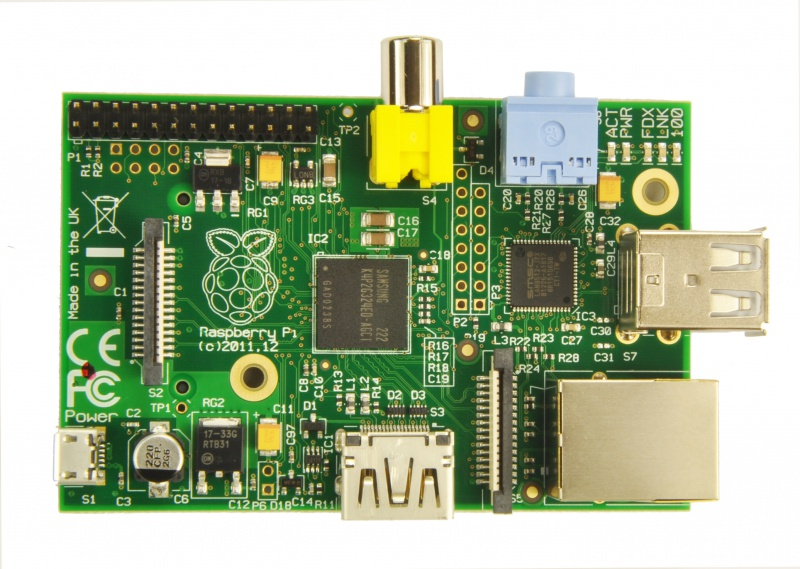
\includegraphics[width=0.5\textwidth]{raspberrypi-front.jpg}
  \caption{Raspberry Pi 1 Model B}
  \label{fig:devboard-raspberrypi}
\end{figure}

\subsection{PandaBoard}
% http://pandaboard.org/
% http://elinux.org/File:PandaBoard_front.png
% wget http://elinux.org/images/4/48/PandaBoard_front.png
% mv PandaBoard_front.png pandaboard-front.png

\begin{figure}[htbp]
  \centering
    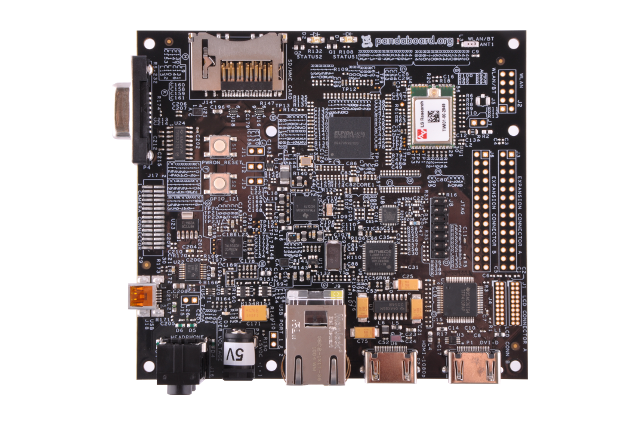
\includegraphics[width=0.5\textwidth]{pandaboard-front.png}
  \caption{Pandaboard}
  \label{fig:devboard-pandaboard}
\end{figure}

drawbacks:\\
- poor support from community\\
- "big" SD card\\
- size: large surface + high audio and Ethernet/USB connectors\\
- Ethernet over USB\\
- serial db-9 connector\\
- strange USB type ab connector\\
- strange graphics solutions (two HDMI s)\\

\subsection{BeagleBone Black}
% https://beagleboard.org/black
% http://elinux.org/File:BeagleBone-Black-A5_product_detail_black_sm.jpg
% wget http://elinux.org/images/a/ac/BeagleBone-Black-A5_product_detail_black_sm.jpg
% mv BeagleBone-Black-A5_product_detail_black_sm.jpg beaglebone-front.jpg

\begin{figure}[htbp]
  \centering
    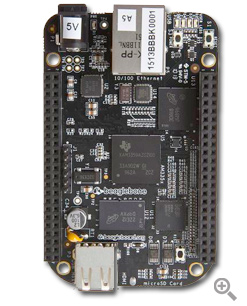
\includegraphics[width=0.25\textwidth]{beaglebone-front.jpg}
  \caption{BeagleBone Black}
  \label{fig:devboard-beaglebone}
\end{figure}

\subsection{Wandboard Quad}
% https://www.wandboard.org/products/wandboard/WB-IMX6Q-BW/
% http://elinux.org/File:Wandboard-dual.jpg
% wget http://elinux.org/images/7/7b/Wandboard-dual.jpg
% mv Wandboard-dual.jpg wandboard-front.jpg

\begin{figure}[htbp]
  \centering
    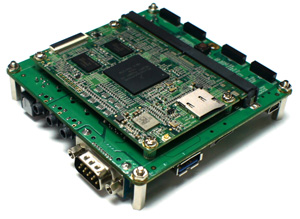
\includegraphics[width=0.5\textwidth]{wandboard-front.jpg}
  \caption{Wandboard}
  \label{fig:devboard-wandboard}
\end{figure}

\subsection{Grinn liteboard}
% http://wiki.litesom.grinn-global.com
% http://linuxgizmos.com/open-spec-sandwich-style-sbc-runs-linux-on-i-mx6ul-based-com/
% wget http://files.linuxgizmos.com/grinn_liteboard.jpg
% mv grinn_liteboard.jpg liteboard-front.jpg

\begin{figure}[htbp]
  \centering
    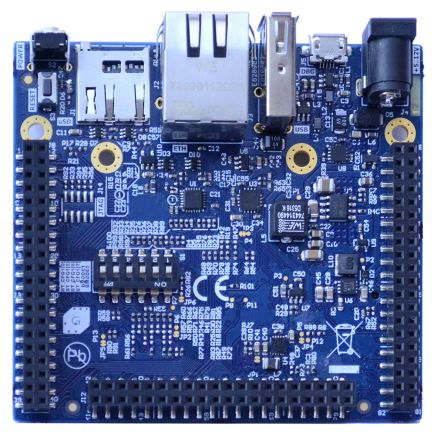
\includegraphics[width=0.5\textwidth]{liteboard-front.jpg}
  \caption{Liteboard}
  \label{fig:devboard-liteboard}
\end{figure}

\subsection{x86\_64 (Asus Eee PC 1215n)}
% https://www.asus.com/Laptops/Eee_PC_1215N/
% https://www.ifixit.com/Guide/Asus+Eee+PC+1215N+Hard+Drive+Replacement/12291
% wget https://d3nevzfk7ii3be.cloudfront.net/igi/eKGfAILyYUfWpePd.medium
% mv eKGfAILyYUfWpePd.medium 1215n-front.jpg

\begin{figure}[htbp]
  \centering
    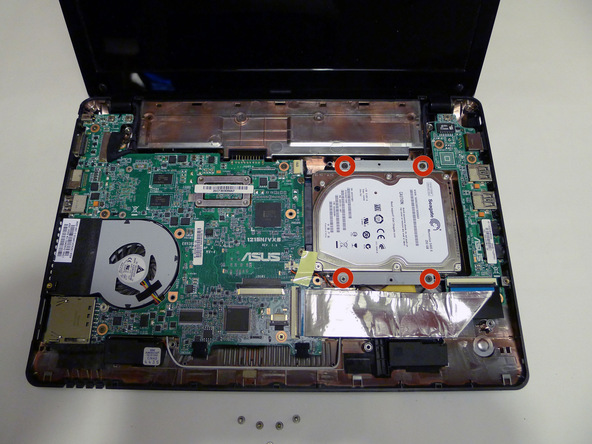
\includegraphics[width=0.5\textwidth]{1215n-front.jpg}
  \caption{Asus Eee PC 1215n}
  \label{fig:devboard-1215n}
\end{figure}


\section{Sources of knowledge}
\label{section:sources-of-knowledge}

There are two important issues, that I faced while making literature review: firstly what kind of materials should I analyze and secondly how to extend my searches, to get a full overview of current state of knowledge on this topic.  \\

First issue was very clear in previous (20th) century - literature review was about analyzing two kind of printed materials: longer ones which were just specialist books and shorter ones which were peer reviewed articles in scientific or industry magazines.
Right now they are also available and easy accessible in electronic form and still they are most reliable sources for literature review, but not every IT engineer is using it.
Open Source Software and Open Source Hardware movement, beside creating loot of tools, also created a lot of written knowledge materials, but they are distributed in very different ways: project documentation, presentations, tutorials, source code comments, READMEs, How Tos, FAQs, wikis, finally blog and forum posts, but also in other forms.
Hopefully, because they are all available via Internet, there exist one unified way to reference them: URL (Unified Resource Locator) also known as web address or link. Because of that, this and most of other bibliographies are filled with URLs, not ISBNs. I tried to divide all of those into groups as clearly as possible.

Second thing is how to be sure that I covered everything, at least by mentioning. Search results are personalized, both by searchers behavior who is choosing keywords and also Search Engine Optimization. Nobody could tell, that this is complete, but sources are cross referenced, so after some research, the loop closed. Most important factor for choosing materials is their universality and chance that they will be not so fast outdated.

\subsection{elinux.org}

The Embedded Linux Developer wiki elinux.org is undeniably the most extensive source of knowledge about all aspects of Embedded Linux.
In this form it was possible to consolidate powerful community which extend its contests.
From one side it is greatly filled with a lot of technical details and still extended, but from the other the content is not always universal and some pages are not maintained.\\

The elinux.org domain was registered on 1999-11-04 \cite{web:whois-elinux} and used by a Linux specialist Tim Riker just as a placeholder \cite{web:riker} \cite{web:elinux-placeholder}.
About 2003 the Embedded Linux wiki was initiated here using MoinMoin framework \cite{web:elinux-moinmoin}.
In 2007 it was moved into Media Wiki engine, that is still in use.
On the top level, its contents are divided into two main parts: "Development Portals" about various aspects of embedded Linux and "Hardware Pages" for different development boards.
The most relevant page for this thesis is \url{http://elinux.org/Build_Systems}, but build systems are only listed there without any comparison.\\

Currently it is maintained by the Core Embedded Linux Project which belongs to Linux foundation \cite{web:linuxfoundation-celp}.
CELP is also coordinator of other important Embedded Linux activities.

\subsection{wikipedia.org}

Although Wikipedia allows anyone to edit articles it is the largest and most popular general reference work on the Internet.
The most important thing from my point of view, is that it redirects and groups abstract entities on the high level.
The table below summarizes pages that are most relevant for this work.

\begin{center}
  \begin{tabular}{| l | l |}
    \hline
    \url{https://en.wikipedia.org/wiki/Category:Embedded_Linux} & \\
    \hline
    \url{https://en.wikipedia.org/wiki/Category:Software_related_to_embedded_Linux} & \\
    \hline
    \url{https://en.wikipedia.org/wiki/Category:Embedded_Linux_distributions} & \\
    \hline
    \url{https://en.wikipedia.org/wiki/Linux_on_embedded_systems} & \\
    \hline
    \url{https://en.wikipedia.org/wiki/List_of_build_automation_software} & \\
    \hline
    \url{https://en.wikipedia.org/wiki/Cross_compiler} & \\
    \hline
    \url{https://en.wikipedia.org/wiki/Microprocessor_development_board} & \\
    \hline
    \url{https://en.wikipedia.org/wiki/Comparison_of_single-board_computers} & \\
    \hline
  \end{tabular}
\end{center}



During this project, I worked on extending enumerated categories and writing first version of article \url{https://en.wikipedia.org/wiki/Embedded_Linux_build_systems}.

It's also possible to process Wikipedia contents and the DBpedia is one of the projects, that aims to transform it into source semantic knowledge.
\begin{itemize}
  \item \url{http://dbpedia.org/page/Category:Embedded_Linux}
  \item \url{http://dbpedia.org/page/Linux_on_embedded_systems%}
\end{itemize}


\subsection{Marcin Bis publications}

In Poland, the most extensive source of written knowledge is provided by Mr Marcin Bis.
He has published two books so far: "Linux w systemach embedded" (eng. "Linux in embedded systems") in 2011 and "Linux w systemach i.MX6 series" (eng. "Linux in i.MX 6 series systems") in 2015.
The company BIS-LINUX.COM also offers various paid workshops and consultations.

\subsection{Conferences and workshops}

From one side there are public events, like Embedded Linux Conferences organized by CELP, from which slides and recordings are available on elinux.org:

\begin{itemize}
  \item \url{http://elinux.org/Category:ELC} - Embedded Linux Conference (America)
  \item \url{http://elinux.org/Category:ELCE} - Embedded Linux Conference Europe
\end{itemize}

Embedded Linux issues connected to build systems are also present on Linux Sessions \cite{web:sesja-linuksowa} coordinated by Academic IT Association from Wroclaw University of Technology. \\

From another side, private companies make mostly interactive workshops. The paid ones are organized i.e. by Marcin Bis \cite{web:bis-szkolenia}. There are also free of charge workshops i.e. ones organized by EBV in 2016, where I participated.

\subsection{scholar.google.com}
% \url{https://www.google.com/?q=embedded+linux+build+systems} (opera + incognito + VPN USA)

The phrase "embedded linux build systems" gives only 2 results  \cite{web:scholar-1}. First of them is presentation "Embedded Linux system development" by Thomas Petazzoni from year 2004. It describes only Open Embedded which is currently included as a part of Yocto Project. Second one is book "Mastering embedded Linux programming" by Chris Simmonds from year 2015. It differentiates only Buildroot and Yocto Project. \\

The phrase "embedded linux build system" gives 24 results \cite{web:scholar-2}. Most of recent works enumerates Buildroot, Yocto Project, OpenWrt without comparison between them. Materials prior to 2010 are mostly using therm "embedded linux distribution", rather than "embedded linux build system".


\subsection{official documentation}

The most valuable source of technical information is and always should be official documentation. URLs are situated in the bibliography and direct to the websites where more information about each project can be found.


\chapter{Creating a basic Linux system}
\label{chapter:basic-system}



\section{Buildroot}



\paragraph{Build procedure}

Buildroot build procedure is the simplest from every point of view.
The only difference between different boards is only \verb|defconfig| name.

\begin{lstlisting}
sudo apt install make gcc g++ libncurses-dev unzip git % patch python rsync bc bzip2 (bzcat)
wget https://buildroot.org/downloads/buildroot-2017.02.9.tar.gz
tar -zxf buildroot-2017.02.9.tar.gz
cd buildroot-2017.02.9/
make raspberrypi_defconfig
make
cp output/images/sdcard.img ..
\end{lstlisting}

% build time

% grabserial -d /dev/ttyUSB0 -m RomBOOT -t -e 30
% ...
% [13.247127 0.001591] buildroot login: 

% # df -h
% Filesystem                Size      Used Available Use% Mounted on
% /dev/root                58.2M     49.6M      4.5M  92% /

% $ du -sh sdcard.img 
% 92M     sdcard.img

% $ du -sh buildroot-2017.02.4
% 4.8G    buildroot-2017.02.4


\section{OpenWrt / LEDE}
% https://lede-project.org/toh/hwdata/raspberrypifoundation/raspberrypifoundation_raspberrypi_bplus
% https://lede-project.org/docs/guide-developer/quickstart-build-images
% https://wiki.openwrt.org/toh/raspberry_pi_foundation/raspberry_pi
% https://lede-project.org/docs/guide-developer/compile_packages_for_lede_with_the_sdk

\begin{lstlisting}
sudo apt install make gcc g++ libncurses-dev unzip git
sudo apt install gawk zlib1g-dev
git clone https://git.lede-project.org/source.git lede
cd lede
git checkout v17.01.2
./scripts/feeds update -a
./scripts/feeds install -a
make defconfig
make menuconfig
Target System (Broadcom BCM27xx)
Target Profile (Raspberry Pi B/B+/CM/Zero/ZeroW)
make -j 12
cp build_dir/target-arm_arm1176jzf-s+vfp_musl-1.1.16_eabi/\
linux-brcm2708_bcm2708/tmp/\
lede-brcm2708-bcm2708-rpi-ext4-sdcard.img ..
\end{lstlisting}



\section{LTIB}
% http://download.savannah.nongnu.org/releases/ltib/
% https://midnightyell.wordpress.com

% https://github.com/midnightyell/RPi-LTIB
% rpm -ivh ... (missing ltib rpi tools)
% http://nongnu.13855.n7.nabble.com/Raspberrypi-toolchain-is-missing-from-gpp-td78878.html

% bash "No such file or directory" (32 / 64 bit...)
% https://askubuntu.com/questions/133389/no-such-file-or-directory-but-the-file-exists
% sudo dpkg --add-architecture i386 , etc...
% debian install 32 bit libz
% 64-bit Debian or Ubuntu : apt-get install zlib1g:i386

% ti_3410.fw ltib
% https://github.com/raspberrypi/linux/issues/112
% https://github.com/raspberrypi/linux/commit/e6ef7f6bbc05fdcd7b1f115bb55a32c176663296
% apply patch... for arch/arm/mach-bcm2708/bcm2708.c and drivers/usb/host/dwc_otg/dwc_otg_driver.c
%
% rpm/BUILD/raspberrypi-linux-118e2d3/drivers/usb/host/dwc_otg/dwc_otg_driver.c

% on ubuntu 14.04 32 bit...
% https://stackoverflow.com/questions/25438455/ltib-installation-woes
% http://nongnu.13855.n7.nabble.com/Linux-Mint-1-6-Can-t-get-rpm-4-0-4-tar-gz-at-ltib-line-834-td75924.html
% http://ftp.rpm.org/releases/historical/rpm-4.0.x/rpm-4.0.4.tar.gz

% /sbin/fdisk -l output/images/sdcard.img
% no bootable flag/not working...
% "wrong fs type, bad option, bad superblock"
% mount sdcard image locally ...
% https://askubuntu.com/questions/445979/how-to-mount-sd-card-image-created-with-dd
% https://en.wikibooks.org/wiki/QEMU/Images#Mounting_an_image_on_the_host

\begin{lstlisting}
sudo apt install make gcc g++ libncurses-dev unzip
sudo apt install rpm bison tcl zlib1g-dev


wget https://github.com/downloads/midnightyell/RPi-LTIB/raspberrypi-tools-9c3d7b6-1.i386.rpm
sudo mkdir -p /opt/ltib/pkgs/
sudo cp raspberrypi-tools-9c3d7b6-1.i386.rpm /opt/ltib/pkgs/

sudo dpkg --add-architecture i386
sudo apt update
sudo apt upgrade
sudo apt install zlib1g:i386
sudo apt install libstdc++6-4.8-dbg:i386


wget http://download.savannah.nongnu.org/releases/ltib/ltib-13-2-1-sv.tar.gz
tar -zxf ltib-13-2-1-sv.tar.gz
cd ltib-13-2-1-sv/
./ltib
Platform choice (Raspberry Pi with BCM2835 SoC)

https://github.com/raspberrypi/linux/commit/e6ef7f6bbc05fdcd7b1f115bb55a32c176663296
rpm/BUILD/raspberrypi-linux-118e2d3/arch/arm/mach-bcm2708/bcm2708.c
rpm/BUILD/raspberrypi-linux-118e2d3/drivers/usb/host/dwc_otg/dwc_otg_driver.c
\end{lstlisting}

\section{PTXdist / DistroKit}
% https://debian.pkgs.org/sid/rt-preempt-nonfree-i386/oselas.toolchain-2013.12.1-arm-1136jfs-linux-gnueabihf-gcc-4.8.2-glibc-2.18-binutils-2.24-kernel-3.12-sanitized_2013.12.1_i386.deb.html
% https://debian.pkgs.org/sid/rt-preempt-nonfree-i386/oselas.toolchain-2016.06.0-arm-1136jfs-linux-gnueabihf-gcc-5.4.0-glibc-2.23-binutils-2.26-kernel-4.6-sanitized_2016.06.0_.deb.html

% only when building all with ./build_all_v2.mk
% http://ptxdist.pengutronix.narkive.com/iZ6AhfNp/pull-request-oselas-toolchain-for-upstream-update-for-gcc-4-4-1-and-binutils-2-20
% ln -s /usr/local/bin/ptxdist p

% http://www.friendlyarm.net/forum/topic/4535 (OSELAS Toolchain)

% (missing) lzop barebox

\begin{lstlisting}
sudo apt install make gcc g++ libncurses-dev unzip git
sudo apt install gawk flex bison gettext python-dev lzop

wget http://public.pengutronix.de/software/ptxdist/ptxdist-2017.06.0.tar.bz2
tar -xjf ptxdist-2017.06.0.tar.bz2
cd ptxdist-2017.06.0
./configure
make
sudo make install
cd ..

# wget http://public.pengutronix.de/oselas/toolchain/OSELAS.Toolchain-2016.06.1.tar.bz2
# tar -xjf OSELAS.Toolchain-2016.06.1.tar.bz2
# cd OSELAS.Toolchain-2016.06.1/
# ptxdist select ptxconfigs/arm-1136jfs-linux-gnueabihf_gcc-5.4.0_glibc-2.23_binutils-2.26_kernel-4.6-sanitized.ptxconfig
# sudo mkdir -p /opt/OSELAS.Toolchain-2016.06.1/
# sudo chown debian:debian /opt/OSELAS.Toolchain-2016.06.1/
# ptxdist go

wget http://debian.pengutronix.de/debian/pool/main/o/oselas.toolchain/oselas.toolchain-2016.06.1-arm-1136jfs-linux-gnueabihf-gcc-5.4.0-glibc-2.23-binutils-2.26-kernel-4.6-sanitized_2016.06.1_amd64.deb
sudo dpkg -i oselas.toolchain-2016.06.1-arm-1136jfs-linux-gnueabihf-gcc-5.4.0-glibc-2.23-binutils-2.26-kernel-4.6-sanitized_2016.06.1_amd64.deb


git clone https://git.pengutronix.de/cgit/DistroKit/
cd DistroKit/
ptxdist platform configs/platform-rpi/platformconfig
ptxdist images
\end{lstlisting}

\section{Yocto / OpenEmbedded}
% https://github.com/lukaszgard/sesja-manifest

\begin{lstlisting}
sudo apt install make gcc g++ unzip git
sudo apt install gawk diffstat texinfo build-essential chrpath

mkdir raspberrypi-yocto
repo init -u ...
repo synch
source poky/oe-init-build-env
vi conf/bblayers.conf
export MACHINE=raspberrypi
bitbake core-image-minimal
\end{lstlisting}

\section{Linux From Scratch}

\chapter{Build process comparison}
\label{chapter:methodology}

\section{Build servers}
minimal requirements vs maximum usable resources\\
1. local machine (laptop)\\
2. cloud server (payed m1.2 x large - count time on various sizes + cost + servery.pl vs Amazon AWS)\\
3. dedicated server (own... Intel Xeon)\\
4. dedicated server (payed)\\
count costs in comparison to... big mac / salary?

% https://github.com/pkgcloud/pkgcloud
% https://www.alibabacloud.com/
% http://kb.arubacloud.com/en/computing/creating-and-configuring-a-cloud-server/partitioning-and-formatting-an-added-hard-drive-linux-debian.aspx



% wget https://raw.githubusercontent.com/tbird20d/grabserial/v1.9.3/grabserial
% chmod +x grabserial
% sudo cp grabserial /usr/local/bin/
% pip install pyserial

% sudo apt install pv

% table stats
% build time (toolchain / rootfs / image...)
% image size (free space... df -h)
% boot time (dhcpd...?)

\paragraph{OpenStack}

% m1.tiny - VCPUs: 1, RAM: 512 MB
% m1.2xlarge - VCPUs: 12, RAM: 16,384 MB

% s1-2 - VCPUs: 1, RAM: 2,000 MB
% b2-30-flex - VCPUs: 8, RAM: 29.3 GB / 30,000 MB

\begin{enumerate}
  \item Login to Horizon panel (https://horizon.serwery.pl)
  \item Select "instances" and "launch instance"
  \item Choose instance name (mgr-builder-X), type (m1.2xlarge), image (Debian 8.4)
  \item Choose or create key pair
  \item Launch instance
  \item Select "volumes" and "create volume" or... just select "Boot from image (creates a new volume)" 
  \item Choose volume name (mgr-volume-X), type (SAS), size (100 GB)
  \item Create volume
  \item Attach volume to instance
\end{enumerate}

\paragraph{ssh}

\begin{enumerate}
  \item identify (\verb|$HOST_KEYS $HOST_USER $HOST_IP $VOLUME_ID|)
  \item Login with (\verb|ssh -i $HOST_KEYS $HOST_USER@$HOST_IP|)
  \item Update system (\verb|sudo apt update && sudo apt upgrade|)
  \item rest is possibly not needed... using home directory
  \item Create partition on volume (\verb|sudo mkfs.ext4 /dev/sdb|)
  \item Mount volume (\verb|sudo mount /dev/sdb /mnt/|)
  \item (\verb|sudo chown debian:debian /mnt/|)
  \item Navigate to mounted directory (\verb|cd /mnt/|)
\end{enumerate}

\section{Deploy image}

\begin{itemize}
  \item \verb|scp|
  \item \verb!pv sdcard.img | dd of=/dev/sdb bs=4M oflag=dsync!
\end{itemize}



\section{Data storage}
WARNING: DEGRADATION OF SD CARDS! (ram file system... and other mechanisms)

% vi board/grinn/liteboard/genimage.cfg
% rm output/images/*
% make uboot-rebuild
% make linux-rebuild
% make



\chapter{Node.js and IoT}

\paragraph{Buildroot}

\begin{lstlisting}
cd buildroot-2017.02.4/
make clean # because of wchar...
make menuconfig
Toolchain -> Enable WCHAR support
Toolchain -> Enable C++ support
Target packages
Interpreter languages and scripting -> nodejs -> NPM for the target
Networking applications -> openssh
Networking applications -> ntp -> ntpd
Libraries -> Database
mysql support -> mysql variant (mariadb) -> mariadb server
\end{lstlisting}

\chapter{Building containers}

%https://docs.docker.com/engine/userguide/eng-image/baseimages/
% http://michaelcoyote.github.io/2015/08/02/lean-container-tricks/
% https://blog.docker.com/2013/06/create-light-weight-docker-containers-buildroot/

meta-eldk/linux-xenomai
\url{https://layers.openembedded.org/layerindex/recipe/8333/}



\chapter{Conclusions}
\label{chapter:conclusions}

%\chapter{CAN and CANopen}

%\chapter{MIPI CSI and OpenCV}

%\chapter{Real time / Xenomai}

%\chapter{POSIX Test Suites}
%https://www.linuxbase.org/download/
%
%\url{https://en.wikipedia.org/wiki/Linux_Standard_Base}
%\url{https://en.wikipedia.org/wiki/Single_UNIX_Specification}
%\url{https://en.wikipedia.org/wiki/POSIX}
%
%https://www.opengroup.org/testing/downloads.html
%https://www.opengroup.org/testing/linux-test/
%https://wiki.linuxfoundation.org/en/Testing
%
%posixtestsuite-1.5.2.tar.gz
%https://sourceforge.net/projects/posixtest/
%http://posixtest.sourceforge.net/
%https://sourceforge.net/p/posixtest/mailman/posixtest-discuss/
%
%\url{https://github.com/search?utf8=\%E2\%9C\%93&q=posixtest}
%\url{https://github.com/juj/posixtestsuite}

\addcontentsline{toc}{chapter}{Bibliography}
\bibliography{embedded-linux-build-systems}

\listoffigures
\listoftables

\end{document}
